\documentclass{ltjsarticle}

\usepackage{amsmath}
\usepackage{amssymb}
\usepackage{amsthm}
\usepackage{ mathrsfs }
\usepackage{enumerate}
\usepackage{bbm}
\usepackage{lipsum}
\usepackage{fancyhdr}
\usepackage{tikz-cd} 
\usetikzlibrary{graphs}
\usepackage{luatexja-ruby} 
\usepackage{graphicx} 
\graphicspath{ {./../../images/} }

\newtheorem{theorem}{定理}[section] 
\newtheorem{proposition}{Proposition}[section] 
\newtheorem{definition}{定義}[section] 
\newtheorem{problem}{問題}
\newtheorem{postulate}{公準}[section] 
\newtheorem{lemma}{Lemma}[section] 
\newtheorem{notation}{Notation}[section] 
\newtheorem{remark}{注釈}[section] 
\newtheorem{corollary}{系}[section] 
\newtheorem{terminology}{Terminology}[section] 
\newtheorem{example}{例}[section] 
\newtheorem{step}{手順} 
\newtheorem{solution}{解答}[section] 
\newtheorem{fact}{事実}[section] 

\DeclareMathOperator{\diam}{diam}
\DeclareMathOperator{\Gal}{Gal}
\DeclareMathOperator{\rank}{rank}
\DeclareMathOperator{\Hom}{Hom}
\DeclareMathOperator{\Dom}{Dom}
\DeclareMathOperator{\Ann}{Ann}
\DeclareMathOperator{\grad}{grad}
\DeclareMathOperator{\Span}{Span}
\DeclareMathOperator{\interior}{int}
\DeclareMathOperator{\ind}{ind}
\DeclareMathOperator{\supp}{supp}
\DeclareMathOperator{\ob}{ob}
\DeclareMathOperator{\Spec}{Spec}
\DeclareMathOperator{\MaxSpec}{MaxSpec}
\DeclareMathOperator{\PreSh}{PreSh}
\DeclareMathOperator{\Sh}{Sh}
\DeclareMathOperator{\Fun}{Fun}
\DeclareMathOperator{\Ext}{Ext}
\DeclareMathOperator{\Aut}{Aut}
\DeclareMathOperator{\Ker}{Ker}
\DeclareMathOperator{\Image}{Im}
\DeclareMathOperator{\Coker}{Coker}
\DeclareMathOperator{\id}{id}
\DeclareMathOperator{\Mod}{Mod}
\DeclareMathOperator{\QCoh}{QCoh}
\DeclareMathOperator{\Coh}{Coh}
%\newcommand*{\name}[\num_arguments][default values]{{\color{#1}\Large #2}}
\newcommand*{\Z}{\mathbb{Z}}
\newcommand*{\Q}{\mathbb{Q}}
\newcommand*{\R}{\mathbb{R}}
\newcommand*{\multivar}[2]{{#1_1,\cdots,#1_{#2}}}
\newcommand*{\localization}[2]{#1_{\mathfrak{#2}}}
\newcommand*{\ringedspacemorph}[1]{(#1,#1^{\#})}
\newcommand*{\sheaf}[2]{(#1,{\mathcal{#2}}_{#1})}
\newcommand{\fib}[1]{%
  \mathbin{\mathop{\times}\limits_{#1}}%
}
\newcommand{\tens}[1]{%
  \mathbin{\mathop{\otimes}\displaylimits_{#1}}%
}
\title{授業ノート}
\author{ボン補習校高校数学}
\date{５月２３日}

\begin{document}

\maketitle

\section{三角関数}

\begin{center}
\begin{tabular}{|l|l|l|}
\hline
           & $\sin$                 & $\cos$                 \\ \hline
$30^\circ$ & ${\frac 1 2}$          & ${\frac {\sqrt{3}} 2}$ \\ \hline
$45^\circ$ & ${\frac 1 {\sqrt{2}}}$ & ${\frac 1 {\sqrt{2}}}$ \\ \hline
$60^\circ$ & ${\frac {\sqrt{3}} 2}$ & ${\frac 1 2}$          \\ \hline
$90^\circ$ & $1$                    & $0$                    \\ \hline
\end{tabular}
\end{center}

ここで$\sin$の微分を考えます。微分の定義を思い出して、$x$における微分は
\begin{equation*}
\lim_{h\to0}{\frac {\sin(x+h)-\sin(x)}{h}}
\end{equation*}
となりますが、$\sin(x+h)$はどのような形をしているのでしょうか。ここで次の定理を証明します。

\begin{theorem}
\begin{equation*}
\sin(a+b) = \sin(a)\cos(b)+\sin(b)\cos(a)
\end{equation*}
\end{theorem}

\begin{center}
\begin{figure}[h]
	\centering
    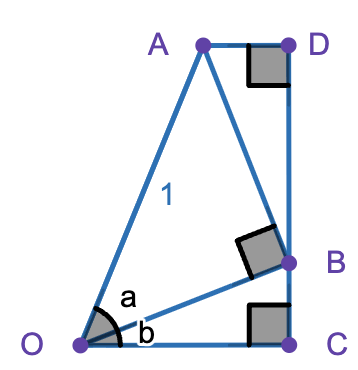
\includegraphics[scale=0.4]{sin_addition}
    \label{fig:Euler_1}
\end{figure}
\end{center}

上の図で点$A$から向かい合う辺$OB$に垂直な線を引き、その交点を$E$とすると$\triangle OAE$は斜辺が$1$の直角三角形で
\begin{equation*}
\angle AOE=a+b
\end{equation*}
となるので、
\begin{equation*}
AE = \sin(a+b)
\end{equation*}
$\square ADCE$は長方形なので
\begin{equation*}
AE = DC = DB+BC
\end{equation*}
なので$DB,BC$の長さをまず求める。
ここで$\triangle BOC$に注目すると
\begin{equation*}
BO = \cos(a)
\end{equation*}
なので
\begin{equation*}
BC = \cos(a)\sin(b)
\end{equation*}
$\triangle ABD$に注目する。一番下の三角形より、
\begin{equation*}
b+\angle OBC+90^\circ  = 180^\circ
\end{equation*}
点$B$の周りに注目して
\begin{equation*}
\angle OBC + 90^\circ + \angle ABD = 180^\circ
\end{equation*}
なので二つの式を比べると、
\begin{equation*}
b = \angle ABD
\end{equation*}
となります。ここで
\begin{equation*}
AB = \sin(a)
\end{equation*}
なことに気をつけ、$\triangle ABD$は直角三角形より
\begin{equation*}
BD = \sin(a)\cos(b)
\end{equation*}
となります。最後に二つを足し合わせて、
\begin{equation*}
AE = DB+BC = \sin(a)\cos(b)+\cos(a)\sin(b)
\end{equation*}
となります。
\par\textbf{問題：}次の計算をしてみよう

\begin{equation*}
\sin(75^\circ)=?,\quad \sin(15^\circ)=?
\end{equation*}
\par\textbf{解答：}\\
\begin{align*}
\sin(75^\circ)& = \sin(30^\circ+45^\circ),\\
& = \sin(30^\circ)\cos(45^\circ)+\sin(45^\circ)\cos(30^\circ),\\
& = 
\end{align*}

次の図を見てみよう。

\begin{center}
\begin{figure}[h]
	\centering
    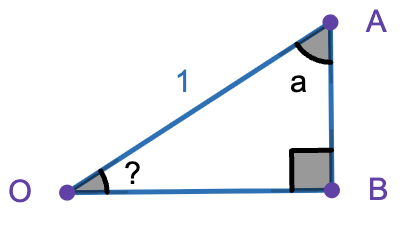
\includegraphics[scale=0.5]{trig_transform}
    \label{fig:Euler_1}
\end{figure}
\end{center}

これを使って$\sin,\cos$の関係を書いてみよう
\begin{equation*}
\cos(x) = \quad\quad,\sin(x)=\quad\quad.
\end{equation*}

さらにこれを使って次のことを証明してみよう。
\begin{equation*}
\cos(x+y) = \cos(x)\cos(y)-\sin(x)\sin(y)
\end{equation*}
今まで習ってきたことを使って次の式を少しだけ簡単にしてみよう。
\begin{equation*}
\lim_{h\to0}{\frac {\sin(x+h)-\sin(x)}{h}}
\end{equation*}

\par\textbf{問題：接線の計算}\\
次の関数の微分を書いて、$x=1$での傾きと、その接線を求めよう。
\begin{equation*}
f(x) = e^x, f(x) = x^2
\end{equation*}
ここで関数$f(x)$の$x=1$での接線は次の式で計算できることを思い出そう。
\begin{equation*}
y-f(1) = f'(1)(x-1)
\end{equation*}

\par\textbf{問題：三倍角の公式}\\
前に習った公式を使うと
\begin{equation*}
\sin(2x) = 2\sin(x)\cos(x),\cos(2x) = \cos(x)^2-\sin(x)^2
\end{equation*}
ということがわかると思います。これを使って次を計算し$\sin(x),\cos(x)$で表しましょう。

\begin{equation*}
\sin(3x),\cos(3x)
\end{equation*}



\end{document}